\documentclass[10pt,conference]{IEEEtran}
\usepackage[T1]{fontenc}
\usepackage{cite}
\usepackage{amsmath}
\usepackage{booktabs}
\usepackage{graphicx}
\usepackage{xcolor}
\usepackage{url}
\usepackage[hidelinks]{hyperref}
\usepackage{pgfplots}
\pgfplotsset{compat=1.17}
\usetikzlibrary{positioning,arrows.meta,fit}

% Marks numbers and text still to come from the running experiments.
\newcommand{\todo}[1]{\textcolor{red}{[TODO: #1]}}
\newcommand{\sys}{\textsc{Ledger}}
\newcommand{\hyb}{\textsc{Ledger+Ep}}

\begin{document}

\title{Facts Where Sure, Episodes Otherwise:\\A Trust-Ranked Bitemporal Ledger for Agent Memory, Evaluated Under Change}

\author{\IEEEauthorblockN{Anonymous Author(s)}}

\maketitle

\begin{abstract}
Agent memory systems are mostly evaluated on questions about a static past,
where retrieving loosely relevant text is enough. Production memory instead
faces facts that change, sources of uneven reliability, and users who ask to
be forgotten. We present \sys{}, a memory layer that stores what an agent
learns as a bitemporal, provenance-tracked ledger of facts, and decides with
explicit rules (restate, supersede, dispute, hold, delete) rather than with
the model which value to trust. A language model only proposes claims; every
claim must be grounded in its source event, and a value from a less trusted
source can neither override nor introduce a fact. \hyb{} adds an episodic
fallback over raw turns for questions the ledger does not model, without
weakening deletion. We evaluate both under one answering model, one prompt and
one price table against no memory, full-history replay and retrieval over raw
transcripts, on LongMemEval and on a generated multi-session coding-agent
workload with planted, typed ground truth. On the coding workload \hyb{}
answers 94.3\% of questions correctly (five seeds), against 82.1\% for full
replay, which sides with stale documents and the agent's own guesses in 45
answers; over 540 days of sessions full replay falls to 70.5\% while \hyb{}
stays above 89\%. When deletion requests are only described, the transcript
baselines send the deleted value to the model in up to 46 probes, our systems
in none. On LongMemEval, \hyb{} matches full replay (74.8\%) with 1\% of its
context. All runs are pinned, cached and replayable.
\end{abstract}

\begin{IEEEkeywords}
LLM agents, agent memory, evaluation, provenance, deletion
\end{IEEEkeywords}

% ---------------------------------------------------------------------------
\section{Introduction}

Coding agents revisit the same repository across hundreds of sessions. What
they need to remember is mostly configuration that \emph{changes}: the
database a service runs on, the branch it deploys from, who is on call. Such
facts are stated in messages, tool output, documents and code changes; they
are updated, restated, contradicted by stale documents and the agent's own
guesses, and sometimes the user asks for one to be forgotten. A memory that
returns the right value next to an outdated one, or brings a deleted value
back, corrupts every later session (Challenge~1 of the call).

The two baselines the call names as hard to beat, full-history replay and
retrieval-augmented generation (RAG) over transcripts~\cite{hu2025memoryagentbench,wu2025longmemeval},
are strong precisely because they keep everything: the right value is almost
always somewhere in the context. That is also their failure mode. Everything
the user ever said, including what was superseded or deleted, reaches the
model, and the model must sort it out on every query. Dedicated memory
systems~\cite{packer2023memgpt,chhikara2025mem0,rasmussen2025zep,xu2025amem}
consolidate, but leave the decision of what is current largely to the model
that writes the memory.

We take the opposite position: \emph{the model proposes, rules decide}. Our
contributions are:
\begin{enumerate}
\item \sys{}, a memory layer that keeps facts as slots with validity
  intervals, provenance and source trust, and applies five explicit write
  rules, so supersession, historical queries, contamination resistance and
  deletion hold by construction rather than by prompt (Sec.~\ref{sec:design}).
\item Three safeguards for LLM extraction found necessary in practice:
  event identifiers enumerated in the output schema, a grounding check that
  drops values absent from their source event, and deletion that does not
  depend on a single routing call. Each removed a measured class of error
  (Sec.~\ref{sec:extraction}).
\item \hyb{}, an episodic fallback that recovers recall on questions the
  ledger does not model while keeping its deletion guarantee
  (Sec.~\ref{sec:hybrid}).
\item An evaluation protocol that scores both the evidence a memory injects
  and the answer a shared model produces from it, types every wrong value
  (stale, future, contaminated, resurrected), and reports cost in dollars,
  tokens, latency and storage under pinned, cached, replayable runs
  (Sec.~\ref{sec:method}), applied to LongMemEval and to a generated coding-agent
  workload (Sec.~\ref{sec:results}).
\end{enumerate}

Table~\ref{tab:req} maps the call's requirements to where we address them.

\begin{table}[t]
\caption{Challenge requirements and where this paper addresses them.}
\label{tab:req}
\centering
\footnotesize
\begin{tabular}{@{}p{0.34\columnwidth}p{0.58\columnwidth}@{}}
\toprule
Requirement & Addressed by \\
\midrule
R1 lifecycle, provenance, deletion, abstention & Ledger rules (\ref{sec:ledger}); evidence carries source events and validity; tombstones; abstention reasons \\
R1 persistence, restarts & Restart after every checkpoint changes no probe (\ref{sec:results}) \\
R2 established benchmark & LongMemEval\_S, stratified subset of 210 questions (\ref{sec:lme}) \\
R2 multi-session agent workload & Generated coding-agent timelines, 5 seeds (\ref{sec:workload}) \\
R2 same model, prompts, budgets & Shared answerer, one token budget, one tokenizer (\ref{sec:protocol}) \\
R2 quality, tokens, \$, ingest, latency, storage & Measured by the runner, never self-reported (\ref{sec:protocol}) \\
R3 checkpoints, degradation, staleness & 8 checkpoints over 540 days; typed errors, store size, latency per checkpoint (Fig.~\ref{fig:long}) \\
R3 pinned, repeated, audited & Pinned snapshots, response cache, 5 seeds $\times$ repeats; 60 judge decisions human-audited, $\kappa=0.97$ (\ref{sec:threats}) \\
\bottomrule
\end{tabular}
\end{table}

% ---------------------------------------------------------------------------
\section{Problem and Invariants}
\label{sec:problem}

We state what a correct memory must do as seven invariants, each with the
failure it rules out:
\textbf{I1 deletion}: a fact the user asked to forget is never returned again,
including for questions about the past (failure: \emph{resurrection}).
\textbf{I2 supersession}: once a fact changes, the old value is no longer the
answer (\emph{stale}).
\textbf{I3 temporal}: ``what held at $t$?'' returns the value at $t$, not a
later one (\emph{future}).
\textbf{I4 deduplication}: restating a fact or re-ingesting an event adds no
item.
\textbf{I5 contamination}: a less trusted source (a stale README, the agent's
guess) does not override the user (\emph{contaminated}).
\textbf{I6 abstention}: with nothing known, say so.
\textbf{I7 isolation}: one user's memory never reaches another.

Every system implements one interface: \texttt{ingest} a batch of events,
\texttt{delete} on request (with or without the source event ids),
\texttt{retrieve} evidence for a query asked at a time, optionally \emph{as
of} an earlier time, within a token budget, or abstain. Systems report the
model usage they consume; the runner, not the system, measures latency,
counts tokens with one tokenizer and converts usage to dollars.

% ---------------------------------------------------------------------------
\section{Design}
\label{sec:design}

\subsection{The ledger}
\label{sec:ledger}

Memory is partitioned by user. A \emph{slot} is a property of an entity,
keyed \texttt{entity/attribute} (e.g.\ \texttt{payments-service/database}).
Each value a slot has held is an \emph{entry} with a validity interval
$[\mathit{from}, \mathit{to})$, the source kind and trust of the event that
set it, and the ids of every event that stated it~\cite{snodgrass1999temporal}.
Sources are ranked: user messages, tool results and code changes 3,
documents 2, assistant messages and tool calls 1. Tool output ranks with the
user because it observes the world (a migration log).

An extractor turns each ingested batch into claims
$\langle\mathit{event}, \mathit{slot}, \mathit{value}\rangle$. The core never
reads free text; it applies one of five rules per claim, in stream order:
\begin{description}
\item[restate] same value as the current entry: add the event to its
  provenance, no new item (I4);
\item[supersede] different value from a source at least as trusted as the
  current entry's: close the current entry at the claim's time, open a new one
  (I2); the closed entry still answers historical questions (I3);
\item[dispute] different value from a less trusted source: kept for audit,
  never retrieved (I5);
\item[introduce] no current value, source trust $\geq 2$: open an entry;
\item[hold] no current value, source trust $< 2$: keep the value as
  \emph{unconfirmed}, never retrieved, until a trusted source states a value.
\end{description}
Table~\ref{tab:example} traces the rules on one fact.

\begin{table}[t]
\caption{The write rules on one slot, \texttt{payments-service/database}.}
\label{tab:example}
\centering
\footnotesize
\begin{tabular}{@{}llll@{}}
\toprule
Day & Source (trust) & Claim & Rule and effect \\
\midrule
1 & user (3) & PostgreSQL 14 & introduce: entry $[1,\infty)$ \\
3 & README (2) & Postgres 12 & dispute: kept for audit only \\
5 & user (3) & PostgreSQL 14 & restate: event added to provenance \\
9 & migrate.log (3) & PostgreSQL 16 & supersede: $[1,9)$ closed, $[9,\infty)$ \\
12 & user (3) & ``forget the database'' & delete: both entries, the dispute \\
 & & & and the events erased; tombstone \\
\midrule
\multicolumn{4}{@{}l@{}}{Asked on day 7: PostgreSQL 14; on day 10 as of day 6: PostgreSQL 14;} \\
\multicolumn{4}{@{}l@{}}{on day 10: PostgreSQL 16; on day 13: abstain, ``deleted at the user's request''.} \\
\bottomrule
\end{tabular}
\end{table}

The \emph{hold} rule closes a gap we found in evaluation: when the extractor
missed the user's first statement, the assistant's later guess
(``I'll assume Mikko Laine is on call'') became the answer. Requiring trust
2 for introduction admits documents, which in practice are often a fact's only
first source; requiring 3 cost 9 correct answers and fixed none
(Table~\ref{tab:ablation}).

\textbf{Deletion} erases every entry, dispute and unconfirmed value of the
affected slots recorded up to the request, leaves a value-free tombstone, and
blocks the source events so a replay cannot bring them back (I1). Affected
slots are those whose entries came from the request's source events or, for a
request given only as text, those the extractor routes the text to
\emph{plus} every slot the text names outright (Sec.~\ref{sec:extraction}).

\textbf{Retrieval} maps the question to known slots and returns, per slot, the
one entry valid at the query's \emph{as-of} time and recorded by the time
asked, as a single line with its validity and source. It abstains with a
reason (``no known slot matches'', ``deleted at the user's request'',
``only an unconfirmed claim'') when there is none (I6). Given correct
claims, evidence therefore never contains a superseded, contradicted or
deleted value; what remains are extraction errors, e.g.\ an update the
extractor missed leaves the old value current.

\subsection{LLM extraction and its safeguards}
\label{sec:extraction}

The LLM extractor makes two structured-output calls: \emph{claims} for each
ingested session, and \emph{route}, which maps a question or deletion request
to slot keys chosen from an enumeration of the user's known slots, so it
cannot invent one. Both calls see the known slots and their current values, so
keys and spellings stay stable. Evaluation exposed three error classes, each
closed by a deterministic safeguard rather than by prompt wording, since
rewording the prompt re-rolls every extraction and moves failures around
(Sec.~\ref{sec:lessons}):
\begin{enumerate}
\item \emph{Mis-copied event ids}: the model wrote \texttt{e0014} for
  \texttt{e00014}, silently dropping a session's claims. The claims schema now
  enumerates the batch's ids (+3.5 points over five seeds).
\item \emph{Ungrounded values}: about one claim in ten was invented, typically
  known values copied onto unrelated events (a diff summary yielded ten
  ``confirmations'') or non-statements turned into values (``not in
  memory''). A claim is kept only if its value occurs in its event, ignoring
  case and punctuation.
\item \emph{Routing misses on deletion}: the router returned no slot for
  ``Don't keep gateway-service's CI provider in memory anymore'' in five of
  five live retries, so the value leaked. Deletion now also erases any
  \texttt{entity/attribute} slot the request names outright (whole-word
  entity, every attribute word prefixing a word of the text).
\end{enumerate}

\subsection{Episodic fallback}
\label{sec:hybrid}

The ledger models facts with one current value. Some questions are not about
such facts: what the assistant recommended, a one-off detail buried in a long
chat, a count across sessions, or a fact whose first statement the extractor
missed. \hyb{} keeps every turn in a transcript store next to the ledger
(Fig.~\ref{fig:arch}) and answers in one of two modes. In \emph{fallback}
mode, the ledger's facts are returned alone whenever it holds any, and
BM25-ranked turns~\cite{robertson2009bm25} only when it holds none; the
evidence stays as clean as the ledger's. In \emph{augment} mode, turns always
fill the budget left after the facts, which come first and carry their
validity; this recovers more detail but brings old values back into the
context, so correctness then rests on the answering model preferring the fact
line. In both modes a question the ledger abstains on because its slot was
deleted gets no turns.

\begin{figure}[t]
\centering
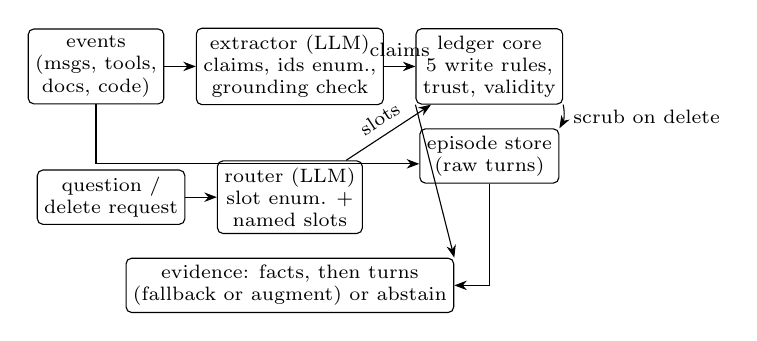
\begin{tikzpicture}[font=\scriptsize, node distance=3mm and 4mm,
  box/.style={draw, rounded corners=2pt, align=center, inner sep=2.5pt, minimum height=5mm},
  ar/.style={-{Stealth[length=1.6mm]}}]
\node[box] (ev) {events\\(msgs, tools,\\docs, code)};
\node[box, right=of ev] (ex) {extractor (LLM)\\claims, ids enum.,\\grounding check};
\node[box, right=of ex] (core) {ledger core\\5 write rules,\\trust, validity};
\node[box, below=of core] (ep) {episode store\\(raw turns)};
\node[box, below=7mm of ex] (rt) {router (LLM)\\slot enum. +\\named slots};
\node[box, left=of rt] (q) {question /\\delete request};
\node[box, below=of rt] (out) {evidence: facts, then turns\\(fallback or augment) or abstain};
\draw[ar] (ev) -- (ex); \draw[ar] (ex) -- node[above]{claims} (core);
\draw[ar] (ev.south) |- ([yshift=-1mm]ep.west);
\draw[ar] (q) -- (rt); \draw[ar] (rt) -- node[above, sloped]{slots} (core);
\draw[ar] (core.south east) to[bend left=20] node[right]{scrub on delete} (ep.north east);
\draw[ar] (core.south west) -- (out.north east);
\draw[ar] (ep) |- (out.east);
\end{tikzpicture}
\caption{\hyb{}: the model proposes claims and routes questions; the ledger
core alone decides what is current, trusted or deleted; the episode store
supplies raw turns and is scrubbed on every deletion.}
\label{fig:arch}
\end{figure}

\textbf{Deletion across both stores.} A raw store can only forget what
something has recognised, so deletion removes from the episodes every event
behind an erased ledger entry, every turn that mentions an erased value,
every turn up to the request that names a deleted slot outright, and every
assistant or tool-call turn up to the request that names an entity the
request is about. The last two rules cover what the ledger never extracted:
an assistant's guess (``Running \texttt{npm test} for inventory-service like
last time'') is no ledger entry under trusted-only extraction, and when the
user's own statement was missed the request matches no slot at all.
Over-deleting the assistant's chatter about a service is the safe direction
for a deletion guarantee; what can remain is a trusted turn the extractor
missed that names neither its value's property nor a value the ledger knew.

\textbf{Trusted-only extraction.} Claims from the assistant could only ever
be held or disputed, so \hyb{} sends only trusted events to the extractor.
On LongMemEval, where 87\% of the history's tokens are the assistant's, this
halves extraction cost with identical accuracy on a 14-question pilot.

% ---------------------------------------------------------------------------
\section{Evaluation Method}
\label{sec:method}

\subsection{Coding-agent workload with planted ground truth}
\label{sec:workload}

A seeded generator produces multi-user, multi-session coding-agent timelines.
Each user owns several services; each service has 3--5 facts drawn from nine
kinds (database, test command, deploy branch, staging host, runtime, message
queue, CI provider, cloud region, on-call owner). A state machine writes each
fact's history as \emph{mutations}: introduce, restate, update, contradict
(from a document or the assistant only) and delete (from the user only).
Every mutation is rendered by a template of its source: user message, tool
output, code diff, document, or assistant message, alongside chit-chat,
tool calls and distractors that name a topic without a value. At four
checkpoints (25--100\% of the stream) the generator asks probes of six types:
\emph{current}, \emph{post-update}, \emph{historical} (with an as-of time),
\emph{contamination}, \emph{post-delete} and \emph{abstention}. Expected
answers are never hand-typed: they are recomputed from the mutations, and a
timeline whose stored expectations disagree refuses to load. Values are unique
per user and never sub-phrases of each other, so a value appearing in evidence
identifies one fact. We use two presets (Table~\ref{tab:workloads}): \emph{small}
for the main comparison and ablations, and \emph{long}, a year and a half of
sessions with eight checkpoints, for behaviour over time. Seeds 5--9 of the
small preset are held out: no design decision was made on them.

\begin{table}[t]
\caption{Workloads. Ranges are over seeds; tokens counted with the runner's
tokenizer over all events.}
\label{tab:workloads}
\centering
\footnotesize
\begin{tabular}{@{}lrrr@{}}
\toprule
 & Small (s0--4) & Long (s0--2) & LongMemEval \\
\midrule
Users (histories) & 3 & 6 & 210 \\
Sessions & 48 & 360 & ${\approx}$48 each \\
Events & 184--218 & 1{,}151--1{,}203 & ${\approx}$493 each \\
History tokens & 2.0k--2.6k & 12.4k--13.2k & 96k--106k each \\
Facts / mutations & 22--34 / 63--105 & 60--81 / 242--329 & -- \\
Deletions & 4--7 & 20--32 & -- \\
Checkpoints & 4 & 8 & 1 per history \\
Probes & 512 in total & 1{,}379 in total & 210 \\
\bottomrule
\end{tabular}
\end{table}

\subsection{LongMemEval}
\label{sec:lme}

LongMemEval\_S~\cite{wu2025longmemeval} has 500 questions, each after a
history of about 48 chat sessions (${\approx}$115k tokens). We draw a
stratified subset with a fixed seed: 30 questions from each of the six types
and 30 abstention questions (210). Each history is replayed session by session
in date order into a fresh store, and the question is asked at its date.
Answers are judged with the benchmark's own prompts, verbatim, on its judge
model \texttt{gpt-4o-2024-08-06} at temperature 0; the only change is that the
judge returns \texttt{yes}/\texttt{no} in a JSON field.

\subsection{Protocol}
\label{sec:protocol}

\textbf{Systems.} No memory; full replay (the whole history, unbounded);
transcript RAG (BM25 over events, top 5, within the budget);
Mem0~\cite{chhikara2025mem0} (OSS release 1.0.11, the last that implements
its published add/update/delete step, unmodified, with a local vector store,
\texttt{text-embedding-3-small} and our extraction model; top 10), and the same
with its list of personal fact types replaced by our extractor's definition of
a coding fact, a prompt fixed before any run (\emph{coding prompt}); \sys{} with a
rule-based extractor (a model-free floor) and with the LLM extractor; and
\hyb{}. Bounded systems share one evidence budget (2{,}000 tokens on the coding
workload, 4{,}000 on LongMemEval); the runner truncates whole items.

\textbf{Shared answerer.} Every system's evidence goes to the same model
(\texttt{gpt-4.1-mini-2025-04-14}, temperature 0, fixed seed) with the same
prompt, memory first and question last. The answer is structured (value,
abstain flag), so on the coding workload abstention is read from a field and
answers are scored deterministically against the planted truth with no LLM
judge.

\textbf{Two scores.} The \emph{evidence verdict} asks what reached the
context: \emph{correct}; \emph{polluted} (right value next to a forbidden
one); \emph{wrong}; \emph{missed}; \emph{false abstention}; and, where the
truth is to abstain, \emph{leaked} (a forbidden value surfaced) or \emph{no
abstention}. Each forbidden value is typed stale, future, contaminated or
resurrected from the fact's mutations. The \emph{answer verdict} applies the
same rules to the shared model's answer. The two differ exactly when the model
repairs or spoils what memory gave it, and a privacy failure (a deleted value
sent to the model) is visible only in the first.

\textbf{Cost and efficiency.} Prices are pinned per model in a table
(USD per million input/output tokens, copied from the provider's model pages
on 2026-10-19); input is charged uncached, an upper bound. We report injected
tokens per question, write-path model calls and tokens, ingest time,
retrieval latency, and store size at each checkpoint.

\textbf{Reproducibility.} Model snapshots and sampling are pinned (temperature
0 and a fixed seed); every response is cached on disk under a hash of
provider, model, prompt and schema, so a run replays at zero cost and every
log records model ids, prompt hashes and counts of cache hits, dropped and
ungrounded claims. Five seeds give variance across workloads; repeated runs
with the cache bypassed measure the model's own noise.

% ---------------------------------------------------------------------------
\section{Results}
\label{sec:results}

\subsection{Coding-agent workload}

\begin{table*}[t]
\caption{Coding-agent workload, small preset, seeds 0--4 (512 probes). \emph{Answer}
and \emph{Evidence}: \% correct, mean $\pm$ sd over seeds. \emph{Wrong ans.}:
answers containing a forbidden value. \emph{Forbidden in evidence}: probes whose
evidence carried a stale / future / contaminated value (a probe can count in several). \emph{Deleted value}:
probes whose evidence / answer contained a deleted value when deletion requests
carry only a description. \emph{Tokens}: mean injected per probe. \emph{\$}: memory
plus answering, all seeds.}
\label{tab:coding}
\centering
\footnotesize
\begin{tabular}{@{}lccrcccr@{}}
\toprule
System & Answer & Evidence & Wrong ans. & Forbidden in evidence & Deleted value & Tokens & \$ \\
\midrule
No memory & 29.5 $\pm$ 1.5 & 0.0 $\pm$ 0.0 & 0 & 0/0/0 & 0 / 0 & 0 & 0.05 \\
Full replay & 82.1 $\pm$ 3.0 & 21.9 $\pm$ 1.8 & 65 & 129/93/93 & 46 / 4 & 982 & 0.28 \\
Transcript RAG & 74.8 $\pm$ 3.6 & 27.0 $\pm$ 5.0 & 88 & 101/69/66 & 39 / 0 & 120 & 0.08 \\
\sys{} (rules) & 39.5 $\pm$ 6.9 & 38.7 $\pm$ 6.3 & 9 & 9/0/0 & 0 / 0 & 4 & 0.05 \\
\sys{} (LLM) & 90.9 $\pm$ 5.5 & 91.7 $\pm$ 5.2 & 4 & 4/0/1 & 0 / 0 & 15 & 0.23 \\
\hyb{} fallback & 94.3 $\pm$ 4.2 & 66.8 $\pm$ 4.6 & 10 & 6/8/3 & 0 / 0 & 56 & 0.23 \\
\hyb{} augment & 94.4 $\pm$ 2.2 & 32.4 $\pm$ 7.8 & 15 & 104/70/60 & 0 / 0 & 133 & 0.25 \\

\bottomrule
\end{tabular}
\end{table*}

Table~\ref{tab:coding} gives the results. Three findings stand out.

\emph{Trust decided by rules beats trust decided by the reader.} With the whole
history in context, full replay answers 82.1\% correctly, but 65 of its answers
contain a forbidden value; 45 of these are \emph{contaminated}: the model sides
with a stale document or with the assistant's own earlier guess over the user.
It answers only 31/67 contamination probes. \sys{} answers 62/67, because
the less trusted claim never reaches the context, and gives 4 wrong answers in
total, all from updates the extractor missed.

\emph{The episodic fallback recovers recall without giving up correctness.}
\hyb{} answers 94.3--94.4\%, the best of all systems, mostly by turning the
ledger's false abstentions on historical questions into answers. In fallback
mode its evidence carries a forbidden value in 16 probes, against 249 for full
replay and 195 for transcript RAG; augment mode carries one in 193, as many as
transcript RAG, so its correctness rests on the answerer preferring the
ledger's fact line, which comes first.

\emph{Deletion must be measured in the evidence.} When deletion requests carry
only a description, the transcript baselines cannot act on them: full replay sends
the deleted value to the model in 46 probes and repeats it to the user in 4;
transcript RAG sends it in 39. At answer level the leak is mostly invisible, since
the model obeys the earlier ``forget it'' message it also sees. \sys{} and \hyb{}
send no deleted value in either mode. An earlier version of \hyb{} did (3 probes):
with trusted-only extraction, an assistant's guess at a value never became a
ledger entry and survived as a raw turn, which motivated the entity-level
scrubbing in Sec.~\ref{sec:hybrid}.

\emph{Held-out seeds.} All design decisions were made while inspecting seeds
0--4. On seeds 5--9, run once with the final systems (Table~\ref{tab:heldout}),
\hyb{} (91.1--91.8\%) and \sys{} (88.2\%) each lose about three points,
while the untuned baselines stay level or rise slightly (full replay 83.3\%,
transcript RAG 78.5\%). The development seeds thus flatter our systems
somewhat; the ordering and the margin over full replay (about eight points)
hold.

\begin{table}[t]
\caption{Held-out seeds 5--9 of the small preset (526 probes), never inspected
during development: answer and evidence accuracy (\%, mean $\pm$ sd over seeds)
and answers containing a forbidden value.}
\label{tab:heldout}
\centering
\footnotesize
\begin{tabular}{@{}lccr@{}}
\toprule
System & Answer & Evidence & Wrong ans. \\
\midrule
No memory & 29.4 $\pm$ 2.9 & 0.0 $\pm$ 0.0 & 0 \\
Full replay & 83.3 $\pm$ 2.8 & 21.1 $\pm$ 0.7 & 58 \\
Transcript RAG & 78.5 $\pm$ 3.1 & 23.8 $\pm$ 3.6 & 81 \\
\sys{} (rules) & 37.0 $\pm$ 2.2 & 37.0 $\pm$ 2.2 & 13 \\
\sys{} (LLM) & 88.2 $\pm$ 3.2 & 89.9 $\pm$ 1.7 & 5 \\
\hyb{} fallback & 91.1 $\pm$ 5.4 & 64.2 $\pm$ 4.8 & 15 \\
\hyb{} augment & 91.8 $\pm$ 4.1 & 25.9 $\pm$ 3.8 & 23 \\

\bottomrule
\end{tabular}
\end{table}

\subsection{LongMemEval}

\begin{table*}[t]
\caption{LongMemEval\_S, stratified subset of 210 questions (30 per category).
Accuracy (\%) with a 95\% bootstrap interval, by category, mean injected tokens,
and cost per question in milli-dollars for memory (write-time extraction, once per
history) and answering. Judge: \texttt{gpt-4o-2024-08-06} with the benchmark's prompts.}
\label{tab:lme}
\centering
\footnotesize
\begin{tabular}{@{}lc ccccccc rrr@{}}
\toprule
System & Accuracy & SS-U & SS-A & Pref & Multi & KU & Temp & Abs & Tokens & Mem m\$ & Ans m\$ \\
\midrule
No memory & 16.2 (11--21) & 0 & 0 & 13 & 0 & 0 & 0 & 100 & 0 & 0.0 & 0.1 \\
Full replay & 74.8 (69--80) & 100 & 97 & 63 & 53 & 90 & 60 & 60 & 108{,}028 & 0.0 & 43.5 \\
Transcript RAG & 71.4 (65--78) & 100 & 97 & 33 & 43 & 73 & 67 & 87 & 1{,}081 & 0.0 & 0.6 \\
Mem0 & 71.0 (65--77) & 83 & 40 & 70 & 53 & 83 & 80 & 87 & 202 & 160.9 & 0.2 \\
\sys{} (LLM) & 41.0 (34--48) & 63 & 3 & 13 & 40 & 60 & 13 & 93 & 13 & 51.0 & 0.1 \\
\hyb{} fallback & 70.5 (65--76) & 97 & 93 & 30 & 50 & 67 & 67 & 90 & 591 & 51.0 & 0.4 \\
\hyb{} augment & 74.8 (69--80) & 97 & 97 & 33 & 60 & 87 & 67 & 83 & 1{,}094 & 51.0 & 0.6 \\

\bottomrule
\end{tabular}
\end{table*}

Table~\ref{tab:lme} shows that on a static, chat-style benchmark the picture
changes. Full replay, now one 108k-token context per question, reaches 74.8\%,
and \hyb{} (augment) reaches the same 74.8\% with 1{,}094 injected tokens, 1\% of
the context; the paired difference is 0.0 points (95\% CI $-6.2$ to $+6.2$). Against
transcript RAG, \hyb{} gains 3.3 points (CI $0.0$ to $+7.1$), concentrated in
knowledge-update (87 vs.\ 73) and multi-session questions (60 vs.\ 43), where
the ledger's current values help; at 210 questions this is borderline. The ledger
alone answers only 41.0\%: LongMemEval mostly asks for one detail buried in
unrelated task chats, and \texttt{gpt-4.1-mini} extracts dozens of incidental
``facts'' per session while missing the needle; by design it also never answers
from the assistant's statements (SS-A 3\%). Full replay is best on
preference questions (63 vs.\ 33), which need the whole conversation's tone rather
than a fact.

\subsection{Over time}

\begin{figure}[t]
\centering
\begin{tikzpicture}
\begin{axis}[name=acc, width=0.56\columnwidth, height=4.2cm, xlabel={checkpoint}, ylabel={answer correct (\%)},
  ymin=60, ymax=100, xtick={1,...,8}, tick label style={font=\scriptsize}, label style={font=\scriptsize},
  legend style={font=\tiny, at={(0.02,0.02)}, anchor=south west, draw=none, fill=none}, legend cell align=left]
\addplot[black, mark=*, mark size=1pt] table[x=cp, y=answer] {figures/long-hybrid_llm_fb.dat};
\addplot[blue, mark=square*, mark size=1pt] table[x=cp, y=answer] {figures/long-ledger_llm.dat};
\addplot[red, mark=triangle*, mark size=1.2pt] table[x=cp, y=answer] {figures/long-full_replay.dat};
\addplot[orange, mark=diamond*, mark size=1.2pt] table[x=cp, y=answer] {figures/long-transcript_rag.dat};
\legend{\hyb{} fb, \sys{}, full replay, RAG}
\end{axis}
\begin{axis}[at={(acc.east)}, anchor=west, xshift=0.9cm, width=0.56\columnwidth, height=4.2cm, xlabel={checkpoint},
  ylabel={probes w/ forbidden evidence}, ymin=0, xtick={1,...,8}, tick label style={font=\scriptsize}, label style={font=\scriptsize}]
\addplot[black, mark=*, mark size=1pt] table[x=cp, y=forbidden] {figures/long-hybrid_llm_fb.dat};
\addplot[blue, mark=square*, mark size=1pt] table[x=cp, y=forbidden] {figures/long-ledger_llm.dat};
\addplot[red, mark=triangle*, mark size=1.2pt] table[x=cp, y=forbidden] {figures/long-full_replay.dat};
\addplot[orange, mark=diamond*, mark size=1.2pt] table[x=cp, y=forbidden] {figures/long-transcript_rag.dat};
\end{axis}
\end{tikzpicture}
\caption{Long preset (6 users, 60 sessions each over 540 days, 8 checkpoints; mean of 3 seeds). Left: answer accuracy per checkpoint. Right: probes per checkpoint whose evidence carried a stale, future or contaminated value.}
\label{fig:long}
\end{figure}

Figure~\ref{fig:long} replays a year and a half of sessions per user. As the
history grows from 549 to 4{,}024 tokens per query, full replay falls from 89.4\%
to 70.5\% and transcript RAG from 88.0\% to 66.5\%, while the forbidden values in
their evidence grow from about 10 to 36 per checkpoint. \sys{} stays between
85.0\% and 93.3\% with about one such probe per checkpoint, and \hyb{}
(fallback) between 89.7\% and 96.2\% with two to four. The ledger's store ends at 1.3\,KiB against 43.5\,KiB for
the transcript stores; \hyb{} keeps both (41.1\,KiB).

\textbf{Restarts.} Snapshotting each store to disk after every checkpoint,
restoring it into a fresh instance and continuing changed no verdict and no
evidence item in any of 1{,}379 probes (3 seeds, 5 systems, 8 restarts each).
Snapshots stay under 270\,KiB and restore in at most 63\,ms.

\textbf{Model change.} Switching \hyb{}'s extraction model from
\texttt{gpt-4.1-mini} to \texttt{gpt-4.1} after the fourth of eight
checkpoints, keeping the store, needs no migration: slot keys and values
written by the old model are routed and restated by the new one. Over two
seeds, accuracy in the second half rises from 92.0\% (mini throughout) to
95.4\%, within 0.3 points of a run on \texttt{gpt-4.1} throughout (95.7\%),
at 62\% of its extraction cost (\$1.18 vs.\ \$1.89 for both seeds).

\subsection{Efficiency and noise}

\begin{table*}[t]
\caption{Efficiency on the coding workload (small preset, seeds 0--4):
write-time LLM calls per ingested session, median ingest time per session and
retrieval time per query, store size at the end per seed, mean injected tokens
per probe, and cost per probe in milli-dollars for memory and for answering.
Times of the LLM systems are from uncached repeats (cached replays are not
timings); augment mode shares fallback's write and routing path. Mem0 with the
coding prompt shares Mem0's embedding cache, so its times are not reported.}
\label{tab:efficiency}
\centering
\footnotesize
\begin{tabular}{@{}lrrrrrrr@{}}
\toprule
System & LLM calls/session & Ingest ms & Retrieve ms & Store KiB & Tokens & Mem m\$ & Ans m\$ \\
\midrule
No memory & 0.00 & 0.00 & 0.00 & 0.0 & 0 & 0.00 & 0.10 \\
Full replay & 0.00 & 0.00 & 0.16 & 8.1 & 982 & 0.00 & 0.55 \\
Transcript RAG & 0.00 & 0.00 & 0.35 & 8.1 & 120 & 0.00 & 0.16 \\
\sys{} (rules) & 0.00 & 0.03 & 0.02 & 0.1 & 4 & 0.00 & 0.11 \\
\sys{} (LLM) & 1.00 & 836 & 666 & 0.4 & 15 & 0.34 & 0.11 \\
\hyb{} fallback & 0.93 & 817 & 662 & 8.0 & 56 & 0.32 & 0.13 \\
\hyb{} augment & 0.93 & 817 & 662 & 8.0 & 133 & 0.32 & 0.16 \\

\bottomrule
\end{tabular}
\end{table*}

Table~\ref{tab:efficiency} gives the cost of the write and read paths. The
LLM systems pay one extraction call per session (0.82--0.84\,s) and one
routing call per question (median 0.66\,s, 95th percentile 0.96\,s); the
transcript systems answer in under a millisecond but inject more context:
982 tokens per probe for full replay and 120 for transcript RAG, against 15
for the ledger and 56 for \hyb{} (fallback). Memory and answering together cost 0.45\,m\$ per probe for \hyb{}
(fallback) against 0.55\,m\$ for full replay, on histories of only a few
thousand tokens. The ledger alone stores 0.4\,KiB per seed against 8.1\,KiB of
transcript.

\textbf{Run-to-run noise.} Three runs per seed of \sys{} and \hyb{}
(fallback) with the response cache bypassed changed the answer verdict of
12 and 8 of 512 probes; the standard deviation of accuracy across repeats is
0.7 and 0.4 points per seed, far below the differences between systems and
seeds reported above.

\subsection{What still fails}

On the coding workload \sys{} fails 47 of 512 probes. Twenty are routing
misses (``no known slot matches''), mostly paraphrases the router does not
link to a slot (``where does it publish its events'' for a message-queue
slot) or slots filed under a short service name (\texttt{inventory/ci\_provider}
beside \texttt{inventory-service/\ldots}). Sixteen are historical questions
asked before the first value the extractor caught: when a fact's first
statement is terse or indirect (\texttt{config-sync: auth.staging\_host =
\ldots}), every earlier as-of question abstains. Four are stale answers from
updates stated indirectly (``build \#812 reported by Jenkins''), the only way
a forbidden value reaches \sys{}'s evidence; two are assistant guesses
correctly held but leaving the question unanswered; and in five the evidence
was right but the answering model abstained. None is a rule applied wrongly.

\hyb{} (fallback) fails 29. The fallback answers most of the ledger's misses
from raw turns, but a raw turn can be old: ten answers carry a stale, future
or contaminated value taken from a turn, and three abstention probes get an
answer where nothing was ever stated. This is the price of the fallback, and
the reason it is used only when the ledger has nothing.

On LongMemEval the dominant failure is recall of a single buried detail: the
ledger alone answers 63\% of single-session-user and 13\% of
temporal-reasoning questions, because \texttt{gpt-4.1-mini} extracts dozens of
incidental ``facts'' per task chat (a quiz's answers, colour codes) and misses
some personal details; preference questions (33\% for \hyb{}) need a summary
of the conversation, which neither facts nor five turns give.

\subsection{Ablations}

\begin{table}[t]
\caption{What changed \sys{}'s evidence accuracy on the coding workload
(5 seeds). The two trust rows replay every extraction from cache, so their
difference is exact; the deletion and grounding rows re-extracted the sessions
whose prompts changed (14 and about 130 live calls).}
\label{tab:ablation}
\centering
\footnotesize
\begin{tabular}{@{}lll@{}}
\toprule
Change & Before & After \\
\midrule
Enumerate event ids in schema & 88.7 $\pm$ 4.0 & 92.2 $\pm$ 4.1 \\
LLM slot-merge check (removed) & 92.2 & 92.0 \\
Terse-value extraction prompt (removed) & 91.9 & 90.7 \\
Neutral router examples & 91.9 & 91.5 \\
\midrule
Hold assistant-first values (trust 2) & 6 wrong & 4 wrong \\
Hold document-first values too (trust 3) & 91.5 & 89.7 \\
Named-slot deletion (description only) & 2 leaked & 0 leaked \\
Grounding check & 1 no-abstention & 0 \\
\bottomrule
\end{tabular}
\end{table}

% ---------------------------------------------------------------------------
\section{Lessons}
\label{sec:lessons}

\textbf{Determinism in rules, not prompts.} With \texttt{gpt-4.1-mini},
rewording the extraction prompt re-rolled about 150 extractions per seed and
moved failures rather than removing them; seeds differ by up to 16 points,
while repeats at temperature 0 flip about two probes per seed. Every lasting
improvement in Table~\ref{tab:ablation} is a deterministic rule.

\textbf{Evidence vs.\ answer.} The answering model repairs much of what
memory gets wrong: full replay's evidence is clean in only 21.9\% of coding
probes, yet 82.1\% of its answers are right, because the model reads dates and
follows the user's corrections. It does so less reliably as history grows
(Fig.~\ref{fig:long}) and not at all for privacy: a deleted value the model
politely does not repeat has still been sent to the provider. Benchmarks that
score only answers cannot see either effect.

% ---------------------------------------------------------------------------
\section{Guidance for Practitioners}
\label{sec:guidance}

\textbf{Which configuration.} Where facts change and sources disagree (coding
agents, operations, account state), \hyb{} in fallback mode gives clean
evidence and the highest accuracy we measured. Where questions are mostly
about one-off details in long chats, augment mode recovers about four points
on LongMemEval at the cost of evidence as noisy as transcript RAG's. The
ledger alone suits uses that must never show an unvetted statement, at the
price of abstaining more.

\textbf{What it costs.} With $c_w$ the write-time cost per history, $c_a$ the
answering cost per question with bounded evidence and $c_f$ full replay's cost
per question, \hyb{} is cheaper after $k > c_w/(c_f - c_a)$ questions per
history: on LongMemEval, $c_w=\$0.051$, $c_a=\$0.0006$ and $c_f=\$0.0435$,
so \hyb{} is cheaper from the second question about the same history, and an
agent working in one repository for months asks many. Extraction cost is
dominated by resending the known slots with every session, not by the
history itself, so it grows with the number of slots and sessions.

\textbf{Operating it.} Every answer is one line per fact with its validity
interval and source, and every abstention has a reason, so a wrong answer can
be traced to the event that set the value or to a routing miss. Disputes and
held claims are kept for audit. Deletion can be verified: after a request, the
slot holds a tombstone and no event stating a deleted value can be ingested
again. Snapshots restore exactly, and the extraction model can be replaced
without migrating the store (Sec.~\ref{sec:results}).

\textbf{What it does not model.} A slot holds one current value, so lists,
counts across sessions and preferences come from the episode store, not from
the ledger. Extraction recall on terse first statements and routing of
paraphrases are the main remaining errors; both are model capabilities, and
the upgrade experiment suggests they improve with the model while the rules
stay unchanged.

% ---------------------------------------------------------------------------
\section{Threats to Validity}
\label{sec:threats}

\textbf{Construct.} The coding workload is generated by us, with templated
phrasings; real traces are messier. Its histories are short (a few thousand
tokens per user), so full replay is cheap there; we did not measure coding
histories beyond 540 days. LongMemEval answers are judged by a model; one
author audited 60 of its decisions (59 distinct responses, as two systems gave
one identical answer), blind to the system (20 each for full replay,
transcript RAG and \hyb{}, half judged correct, spread over all categories).
The judge agreed on 59 (98.3\%, Cohen's $\kappa=0.97$); in the one
disagreement, a preference question answered by transcript RAG, it was
stricter than the human. The auditor noted that the binary judgement accepts
answers that are correct but vague or only partly specific, for every system
alike.

\textbf{Internal.} The ledger's rules and safeguards were developed while
inspecting failures on small-preset seeds 0--4, which we also report; seeds
5--9 are held out and lower our systems' accuracy by two to three points
(Table~\ref{tab:heldout}). The
choice between fallback and augment modes was made on a 14-question
LongMemEval pilot before the main run, and both modes are reported. Runs are
cached, so reported numbers replay exactly; repeated uncached runs put the
model's own noise at under one point per seed (Sec.~\ref{sec:results}).

\textbf{External.} Extraction, routing and answering use one model family
(\texttt{gpt-4.1-mini}, with \texttt{gpt-4.1} in the upgrade experiment), and
all text is English. The LongMemEval subset is 210 of 500 questions, drawn
stratified with a fixed seed; differences of a few points between systems on
it are within its confidence intervals. Besides the baselines the call
requires we compare against one memory product, Mem0, and only on the coding
workload; Zep and A-MEM are not evaluated.

% ---------------------------------------------------------------------------
\section{Related Work}

MemGPT~\cite{packer2023memgpt} pages context like an operating system,
Mem0~\cite{chhikara2025mem0} runs an extract-and-update pipeline,
Zep~\cite{rasmussen2025zep} keeps a temporal knowledge graph, and
A-MEM~\cite{xu2025amem} links notes into an evolving network; reflection
streams~\cite{park2023generative}, skill and workflow
libraries~\cite{wang2023voyager,wang2024awm} and hippocampal
indexing~\cite{gutierrez2024hipporag} extend recall. LoCoMo~\cite{maharana2024locomo},
LongMemEval~\cite{wu2025longmemeval} and MemoryAgentBench~\cite{hu2025memoryagentbench}
measure it. Our ledger is closest to Zep, which also tracks when facts held, but
decides trust, supersession and deletion with explicit rules, and our
evaluation differs in typing each wrong value by why it is wrong and in
scoring the injected evidence as well as the answer.

% ---------------------------------------------------------------------------
\section{Conclusion}

Deciding what memory holds with explicit, auditable rules, and using the
model only to propose and route claims, gives agent memory properties that
replaying or searching transcripts cannot: no stale, contaminated or deleted
value in the context, accuracy that holds as history grows, and restarts and
model changes that change nothing they should not. An episodic fallback
recovers the recall that structured facts give up, at a small fraction of full
replay's context. Code, workloads, pinned prices and all run logs are
available at \todo{anonymous artifact URL}.

\bibliographystyle{IEEEtran}
\bibliography{refs}

\end{document}
